\chapter{绪论}
自从进入21世纪,互联网已经不仅成为人类不可分割的一部分,也成为越来越多设备不可缺少的功能。人类和设备对上网带宽的需求越来越大,这促进了信息技术领域的高速发展。为了满足人类和设备日益增长的带宽需求,光通信已经从主干网逐渐渗入到了房内。而在不远的将未来,光通信将迈向最后一步进入到处理器内部。而这对光通信的器件设备提出了新的要求。


传统光器件,虽然性能满足要求,但是由于其价格高,尺寸大,功耗大将无法满足大规模的应用。因此,研究人员从各方面不断尝试新的材料,新的结构探索高速,小尺寸,小功耗,价格低廉的解决方案。目前这个研究领域依旧热火朝天的进行着。


本章首先将介绍最有希望帮助光通信迈向最后一步的硅基光电子集成技术,接着着重讨论硅基光电子器件中的硅基光调制器,介绍其目前国内外的发展现状,最后将介绍在光调制器领域内由本作者首次完成的工作。


\section{硅基光电子集成技术的发展与现状}
随着信息技术的发展,短距离通信的速率不断提高。当数据的通信速率达到10 Gbps以上时,利用金属的电互联技术将会遇到能耗,串扰,损耗和电磁干扰等问题。尤其,面对当前云计算服务器间和多核处理器内,数据的交互需要在有限的空间内同时满足大带宽、低能耗和低成本的困境时,电互联的瓶颈凸显出来。电互联的这些缺点,可以通过光通信技术来解决。然而传统光通信由于单个光器件的成本高,集成度低,阻碍了传统光通信技术在短距离通信中的应用。

\begin{figure}[htb]
	\centering
	%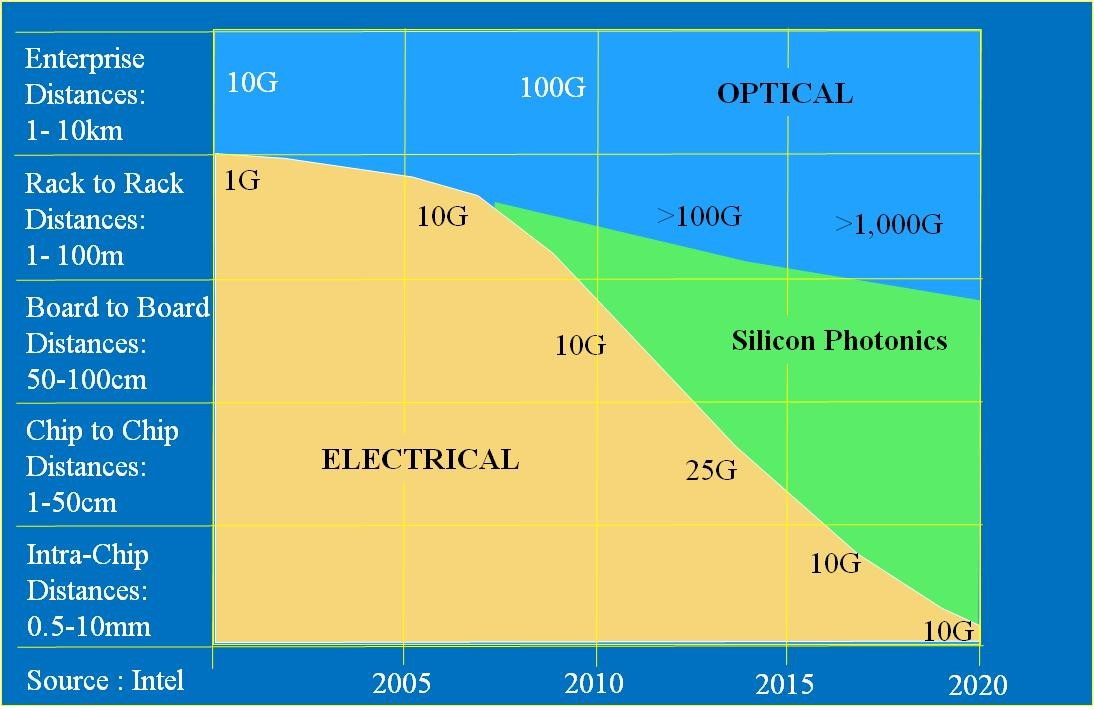
\includegraphics[width=\textwidth]{./Pictures/figure1.jpg}
	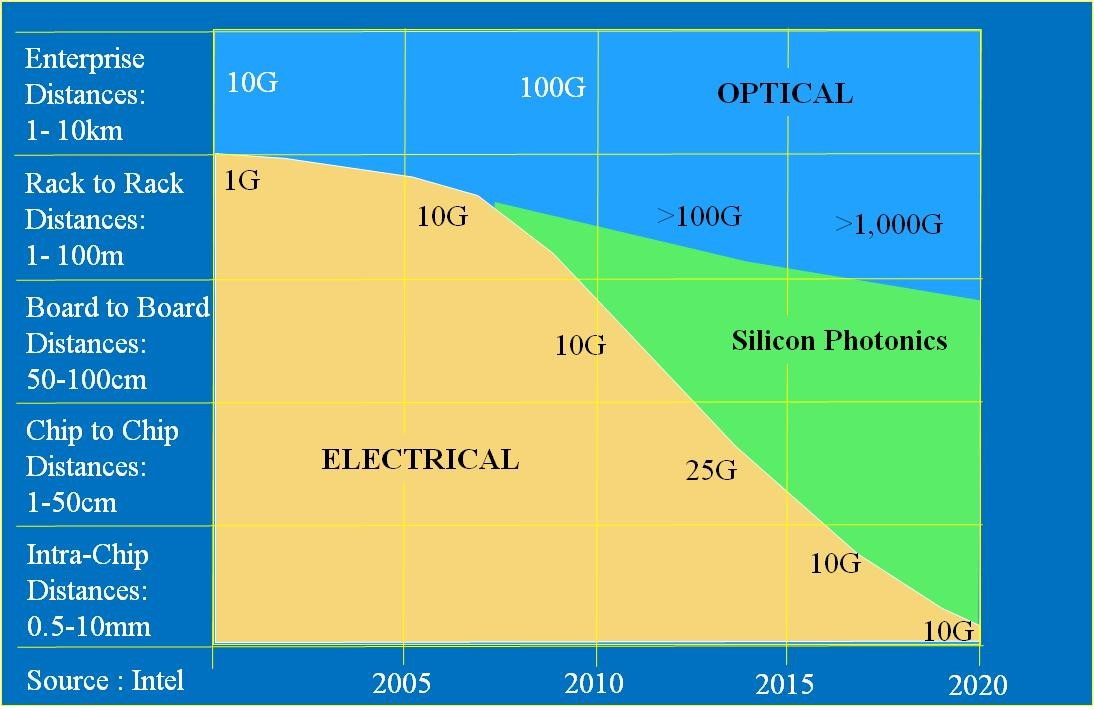
\includegraphics[width=12cm]{./Pictures/figure1.jpg}
	\caption{在不同通信距离下,电互联、硅基光通信和光纤通信的速率使用范围 \cite{Zuffada2012}}
	\label{figure1}
\end{figure}

硅基平台(Silicon-On-Insulator),即由硅衬底、二氧化硅绝缘层和硅薄膜构成的平台,不仅在传统半导体电子领域中有广泛运用,在微纳光子系统中也被广泛采用。硅基平台也成为了实现光电子集成芯片的理想平台。虽然,过去基于III-V材料的InP平台光电子平台已经实现了复杂的通信系统\cite{Meint2014an},比如片上波分复用的光收发器和多波长路由器,但是大规模应用需要价格低廉。除此之外,InP平台上的波导,垂直方向折射率差小只有1\%,导致波导的宽度和高度尺寸在工作波长量级。而硅基光波导在水平和高度方向都有将近60\%的高折射率差,因此光波导尺寸小。又因为硅基平台晶片的单位面积成本比InP晶片低,尺寸又比InP晶片大,所以硅基平台单个光器件的成本远小于InP平台。此外,硅基平台的小尺寸波导传输损耗最低达到 0.4 dB/cm \cite{Tsuyoshi2016low} 小于InP波导的最低传输损耗约为 1 dB/cm \cite{Meint2014an}。从而,硅基光电子平台越来在光通信领域受到人们的关注。

硅基光通信模块作为硅基光电子集成芯片的一个重要应用方向,其具有带宽大,功耗低,成本低的特点。图 \ref{figure1} 描述了电互联、硅基光通信和传统光纤通信和在不同距离下的适用速率范围 \cite{Zuffada2012}。图 \ref{figure1} 也预测了随着通信速率的逐年提高,硅基光通信在短距离将逐渐代替电互联。因此,硅基光集成芯片越来越受到各国的关注。美国在2004年率先提出了EPIC (Electronic and Photonic Integrated Circuits on Si)计划,研究硅基光电子集成平台,这将有助于通信,传感,微波光子学等研究方向的发展\cite{Shah2005}。欧洲在2008年提出了HELIOS (pHotonics ELectronics functional Integration on CMOS)计划,研究基于CMOS工艺的硅基光电子平台 \cite{HELIOS}。日本也紧跟而上,在2010年提出了PECST(Photonics and Electronics Convergence System Technology),推动硅基光电子平台的发展,实现芯片间的通信带宽密度达到10 Tb/s/cm\SP{2}\cite{Arakawa2013Silicon}。

光集成芯片的概念最早是由美国贝尔实验室的Miller在1969年提出来的\cite{miller1969}。随后1993, 美国空军科学研究实验室的Richard A. Soref提出了的硅基光电子集成芯片的概念\cite{Soref1993},见图 \ref{figure2} (a). 硅基光电子芯片是在同一片硅衬底上集成了负责逻辑和驱动的晶体管,负责光通信的激光器,调制器,光放大器,光探测器,光无源结构,光波导和光纤的耦合结构。在接下来的20多年内,全世界的知名高校和半导体公司都投入大量资金到这个领域中。在2011年,见图 \ref{figure2} (b), Intel厚积薄发推出了世界上第一款硅基光通信芯片包含了片上的激光器,纯硅调制器和硅锗探测器的光通信模块,实现了单通道12.5 Gbps的传输速率 \cite{Paniccia2011}。在2012年,见图 \ref{figure2} (c, d), IBM紧接发布了利用改进的90 nm CMOS工艺线,实现了在单个硅片上同时集成晶体管和的25 Gbps的光调制器和探测器 \cite{Assefa2012}。Intel虽然集成了激光器但是没能在单片上同时集成晶体管,而IBM虽然集成了晶体管,却没能集成激光器并且缺少完整光收发链路的展示。在2015年,美国伯克利大学和麻省理工大学的Chen Sun等首次展示了直接在商业化的45 nm CMOS流水线上,制作硅基光电子集成芯片 \cite{sun2015single}。该单块芯片,见图\ref{figure3} (a), 上不仅包含处理器,内存,还包含光收发模块。并且他们还展示了如图 \ref{figure3} (b) 所示的处理器的芯片和内存的芯片直接用光互联技术进行时时数据的运算和处理。虽然该硅基光电子芯片依旧缺少片上的激光器和放大器,但是该芯片是目前最复杂的单片硅基光电子芯片,包含了700万个晶体管和850个光模块。

\begin{figure}[htb]
	\centering
	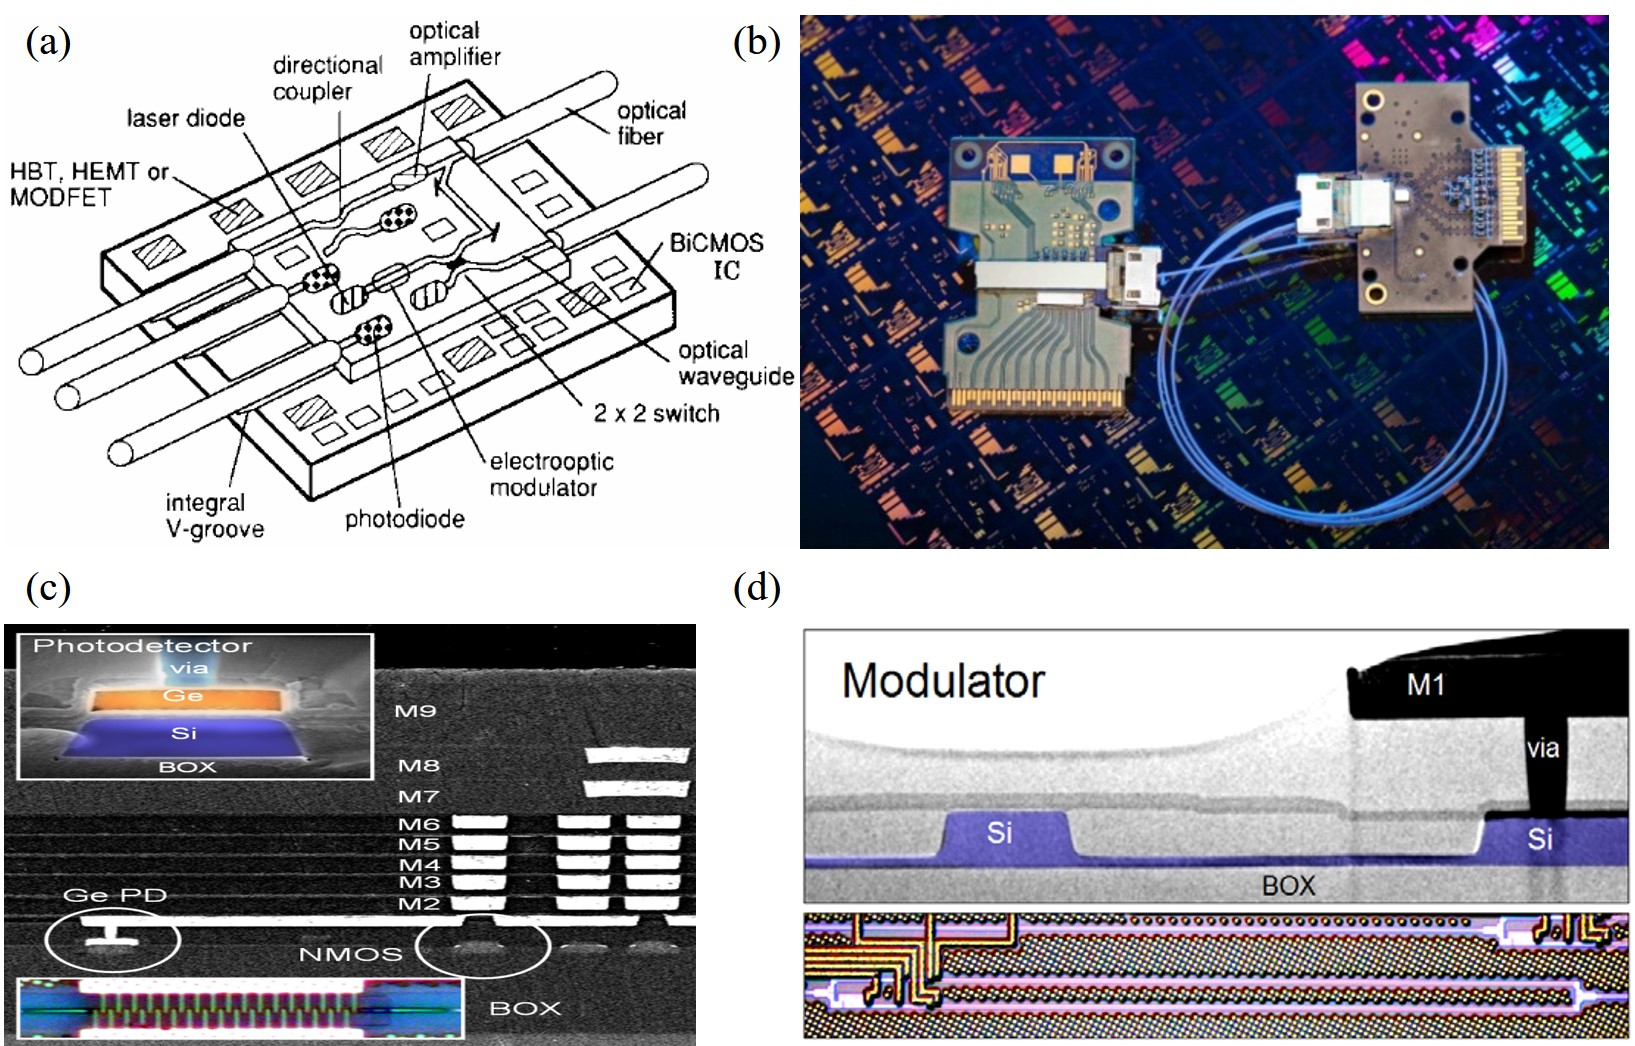
\includegraphics[width=12cm]{./Pictures/figure2.jpg}
	\caption{ (a) 最早的硅基光电子芯片概念图 \cite{Soref1993};(b)Intel的硅基光收发模块\cite{Paniccia2011};(c,d) IBM的硅基探测器和调制器\cite{Assefa2012}}
	\label{figure2}
\end{figure}

\begin{figure}[htb]
	\centering
	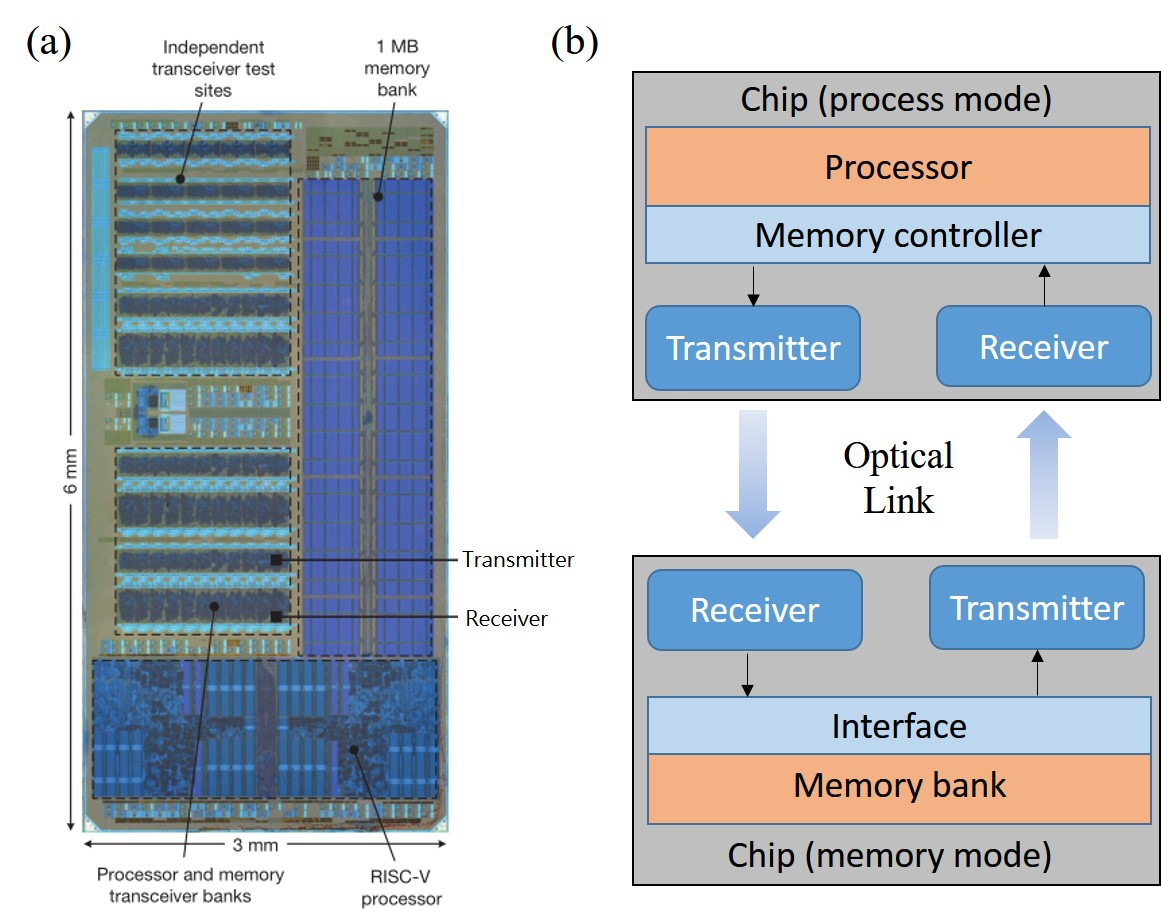
\includegraphics[width=10cm]{./Pictures/figure3.jpg}
	\caption{ (a) 单片硅基光电子芯片,包含处理器,内存,光收发模块\cite{sun2015single};(b) 处理器芯片和内存芯片间光互联示意图}
	\label{figure3}
\end{figure}

\section{硅基光调制器}
硅基光调制器做为硅基光通信模块中不可缺少的一环,连接了电信号向光信号的转化,影响着光通信模块的通信速度和能耗,一直硅基光通信领域的重点和难点。下面将讨论目前硅基光调制器在光学结构和电学结构的研究成果,概括不同材料在硅基平台上实现光调制器的最新进展。
\subsection{硅基光调制器的光学结构}
硅基光调制器如同传统的光调制器,是利用电信号改变材料折射率的实部或者虚部,从而调制器光信号的相位或者幅度。材料的折射率可以用可以表示为:
\begin{equation}
	\label{Equ:index}
	\widetilde{n(\lambda)} = n(\lambda) + j\kappa(\lambda) =  n(\lambda) + j\frac{\lambda\alpha(\lambda)}{2\pi}
\end{equation}
其中$n$为材料折射率的实部,$\kappa$为材料折射率的虚部(称作消光系数)。$\alpha$是材料单位长度的损耗。$n, \kappa, \alpha$都是和波长相关。其中$\kappa$和$\alpha$是线性关系。$n$和$\kappa$可以用通过Kramers-Kronig联系到一起。

\begin{figure}[htb]
	\centering
	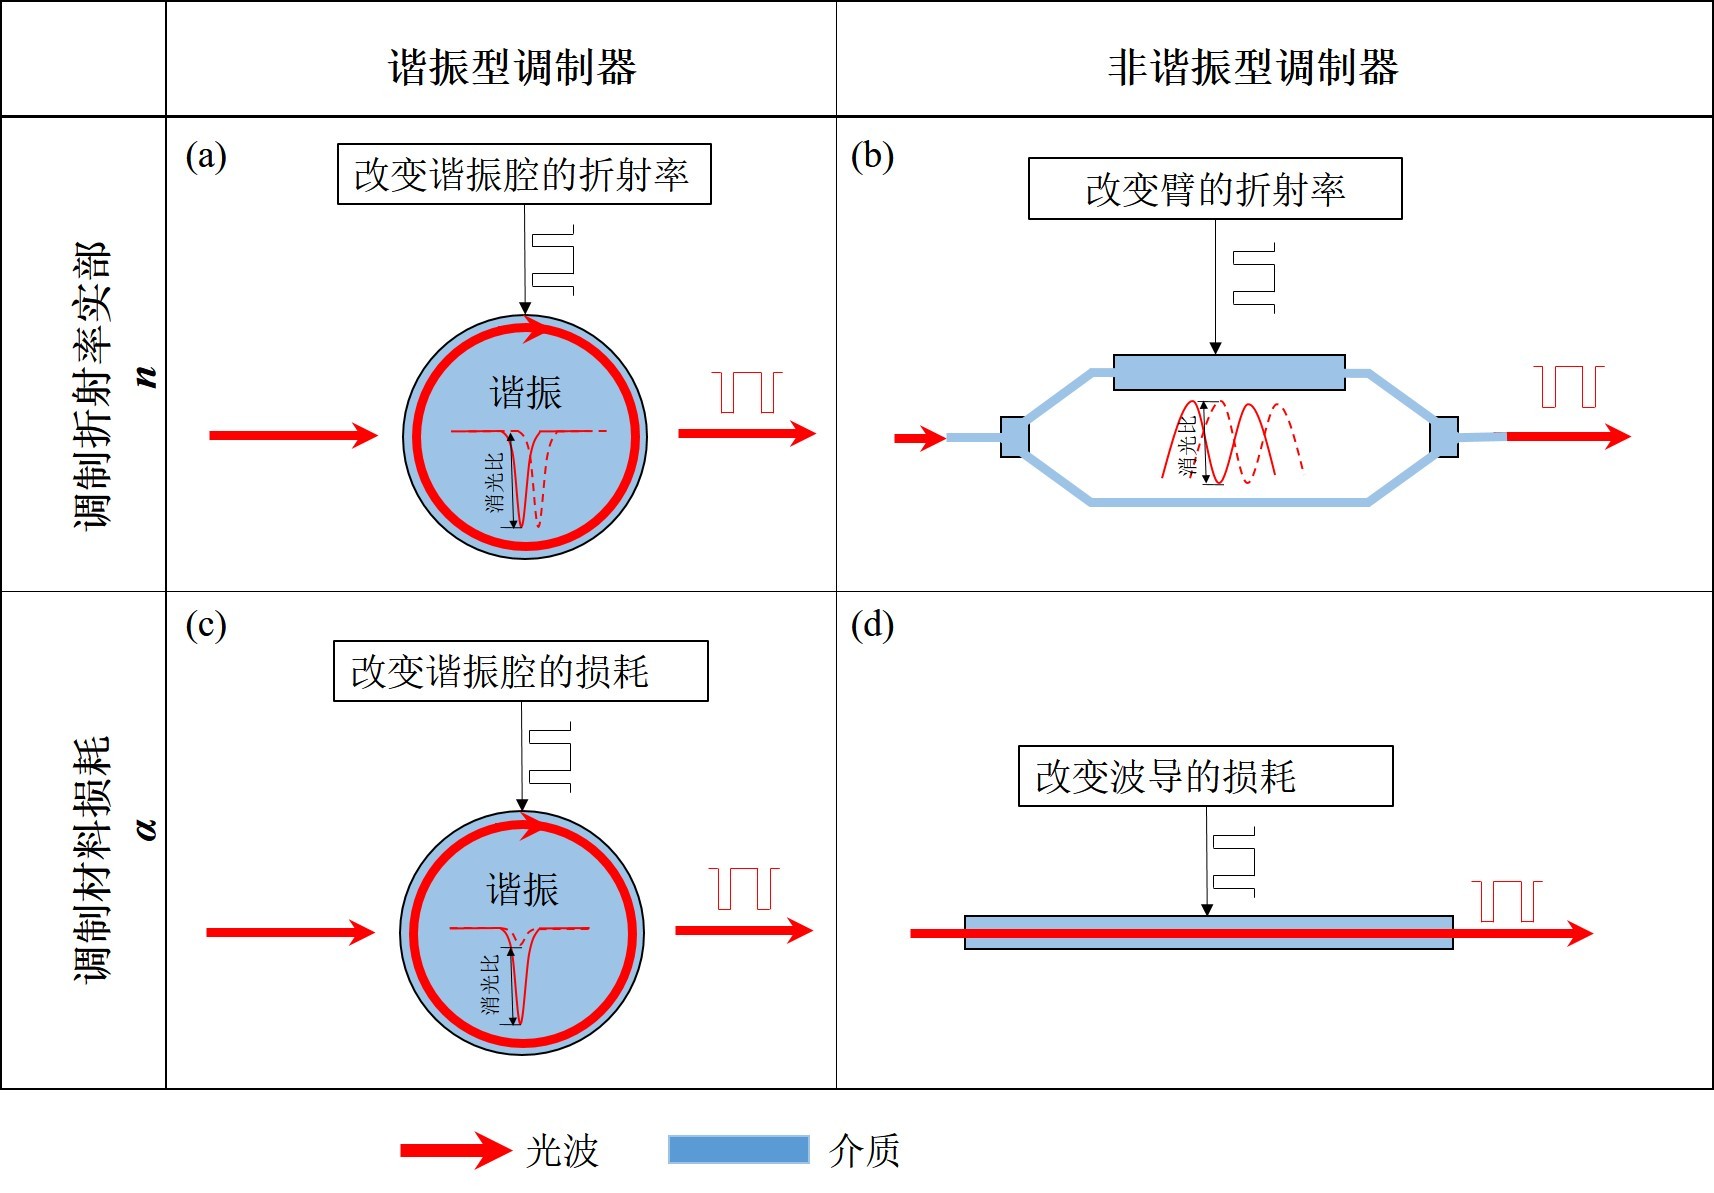
\includegraphics[width=12cm]{./Pictures/fig_mod_opt_type.jpg}
	\caption{ (a, b) 分别是通过调制折射率实部的谐振和非谐振型光调制器;(c, d)分别是通过调制材料损耗的谐振和非谐振型光调制}
	\label{fig_mod_opt_type}
\end{figure}
图 \ref{fig_mod_opt_type} 概括了硅基光调制器的光学结构的四大类型。前两类都是利用电光效应改变光的相位,再利用光学结构转化为光强度的变化。后两类是利用电吸收效应直接改变光的强度。

第一类如图\ref{fig_mod_opt_type} (a) 所示,通过调制折射率实部,改变谐振波长的位置,实现特定波长的调制。这类调制器的特点是结构紧凑,速度快,驱动电压小,能耗低。图\ref{fig_mod_opt_type_real} (a) 展示了最早利用这种结构实现的硅基光调制器的实例\cite{xu2005micrometre}。该调制器利用载流子注入效应,调制硅波导的折射率,移动微环的谐振峰,从而实现谐振波长处光强的调制。

第二类如图\ref{fig_mod_opt_type} (b) 所示,也是通过调制折射率实部,实现相位的调制。这类调制器但是利用马赫曾德结构,将一根波导上的相位变化,转变成强度调制器。其特点是速度快,光学带宽大。图\ref{fig_mod_opt_type_real} (b) 展示了最早利用这种结构的硅基光调制器实例\cite{liu2004high}。该调制器也是利用载流子注入效应,实现马赫曾德一臂的相位变化,从而调制输出的光强。

第三类如图\ref{fig_mod_opt_type} (c)所示,通过调制微环的损耗,从而影响微环的谐振波长处的临界耦合系数,从而调制谐振波长的强度。这类调制器的特点是结构紧凑,驱动电压低,能耗低,速度快。图\ref{fig_mod_opt_type_real} (c) 展示了最早利用这种结构的硅基光调制器的实施方案\cite{Midrio2012graphene}。该调制器利用微环中部分硅波导上的石墨烯,调制石墨烯的损耗,导致微环损耗的变化,从而调制谐振波长处光的强度。由于这类调制器是最近2012年才提出的,目前只在氮化硅平台上有实例\cite{phare2015graphene},在硅基平台上没有实例,只有理论分析的结果\cite{Midrio2012graphene}。

第四类如图\ref{fig_mod_opt_type} (d)所示,直接通过改变波导的损耗,实现光强度的调制。这类调制器的特点是结构紧凑,能耗低,速度快,光学带宽大。图\ref{fig_mod_opt_type_real} (d) 展示了利用这种结构的硅基光调制器实例\cite{tang201150}。该调制器是将InP混合集成到硅波导上,再利用InP多量子阱材料(Multiple Quantum Well, MQW)中量子束缚Stark效应(Quantum Confined Stark Effect, QCSE)实现在不同电压下,材料吸收峰的移动,导致波导的损耗的变化,从而实现光强度的变化。

这四类调制器中的马赫曾德结构除了能用于将光的相位变化转变成强度变化外,还经常被用于高级调制码型的发生器,比如文献[\citenum{Dong2012coherent}]中就利用马赫曾德结构实现正交相移键控(Quadrature Phase-Shift Keying, QPSK)调制码形,并且结合了偏振复用,使单通道的调制速度提高到112 Gbps。
\begin{figure}[htb]
	\centering
	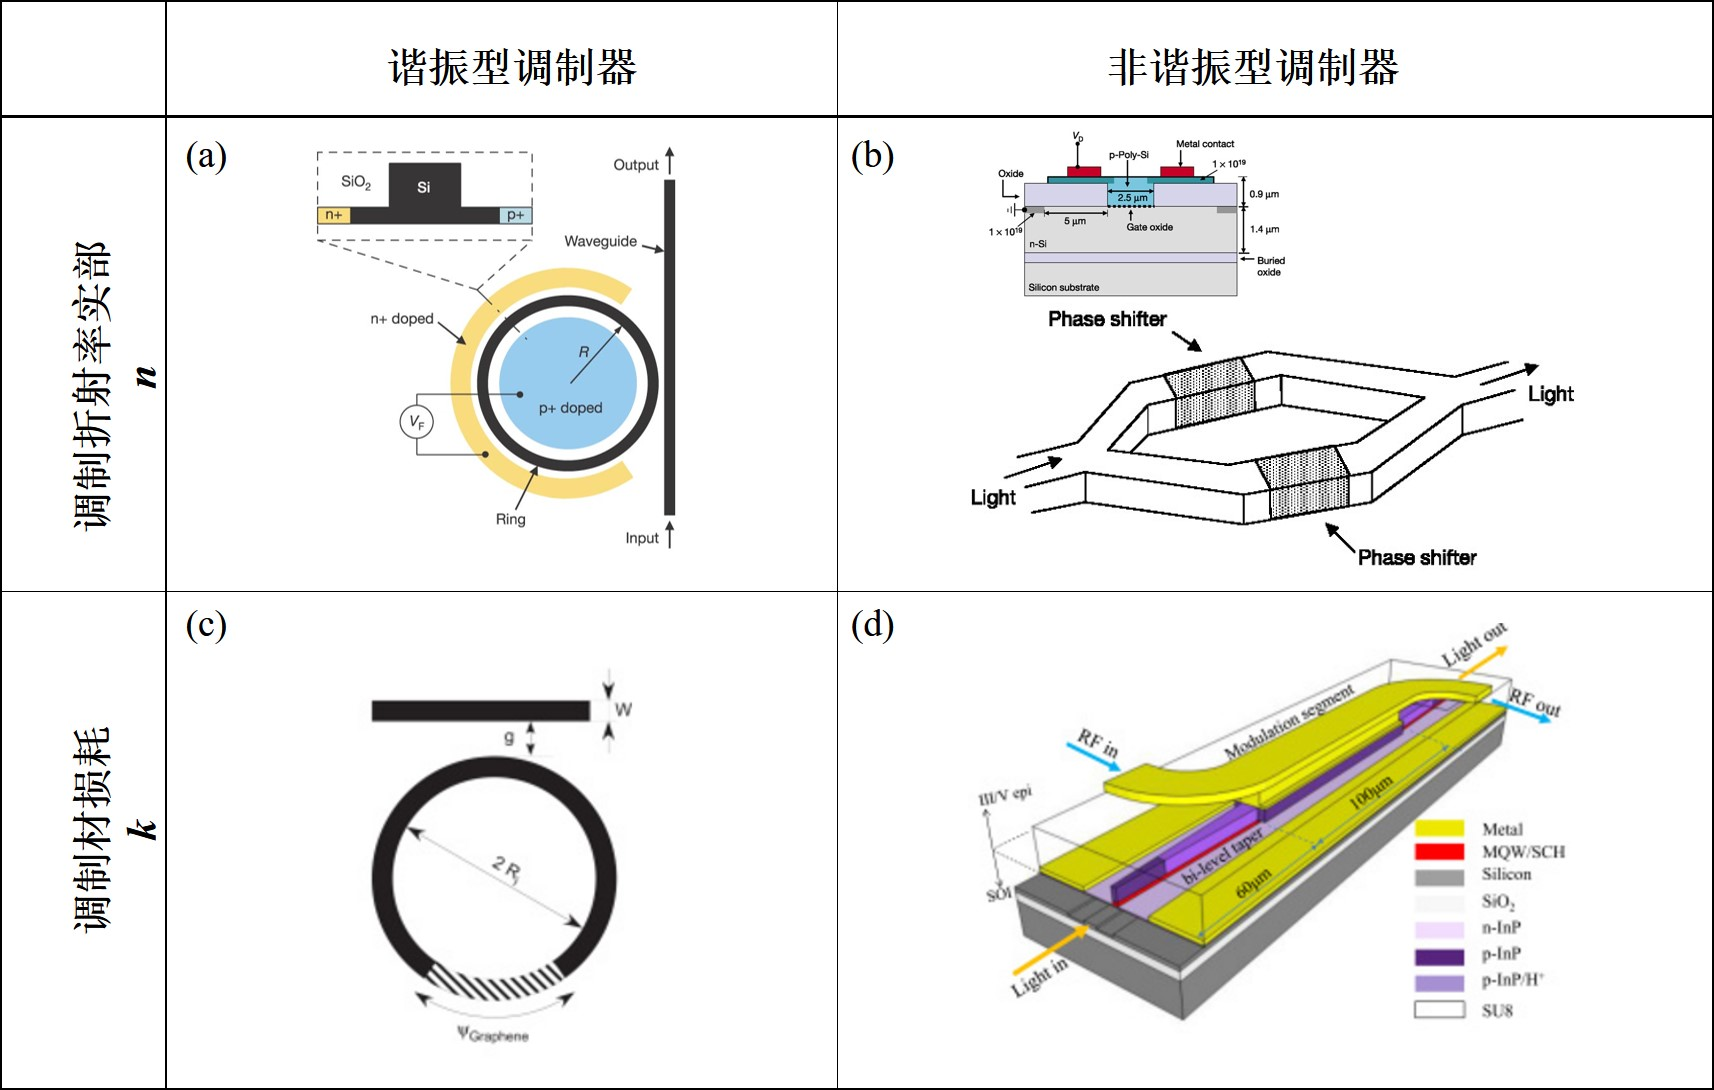
\includegraphics[width=12cm]{./Pictures/fig_mod_opt_type_real.jpg}
	\caption{ (a, b) 分别是通过调制折射率实部的谐振和非谐振型光调制器的实例\cite{xu2005micrometre,liu2004high};(c, d)分别是通过调制材料损耗的谐振和非谐振型光调制的实例\cite{Midrio2012graphene,tang201150}}
	\label{fig_mod_opt_type_real}
\end{figure}

\subsection{硅基光调制器的电极结构}
硅基光调制器的电极结构对调制速率和能耗也有很大影响。图\ref{fig_mod_ele_type}展示了目前硅基光调制器所有的四种电极结构。这四种电极结构已经在InP光调制器和LiNbO\SB{3}光调制器上被广泛应用。下面将讨论这四种电极结构特点。

\begin{figure}[htb]
	\centering
	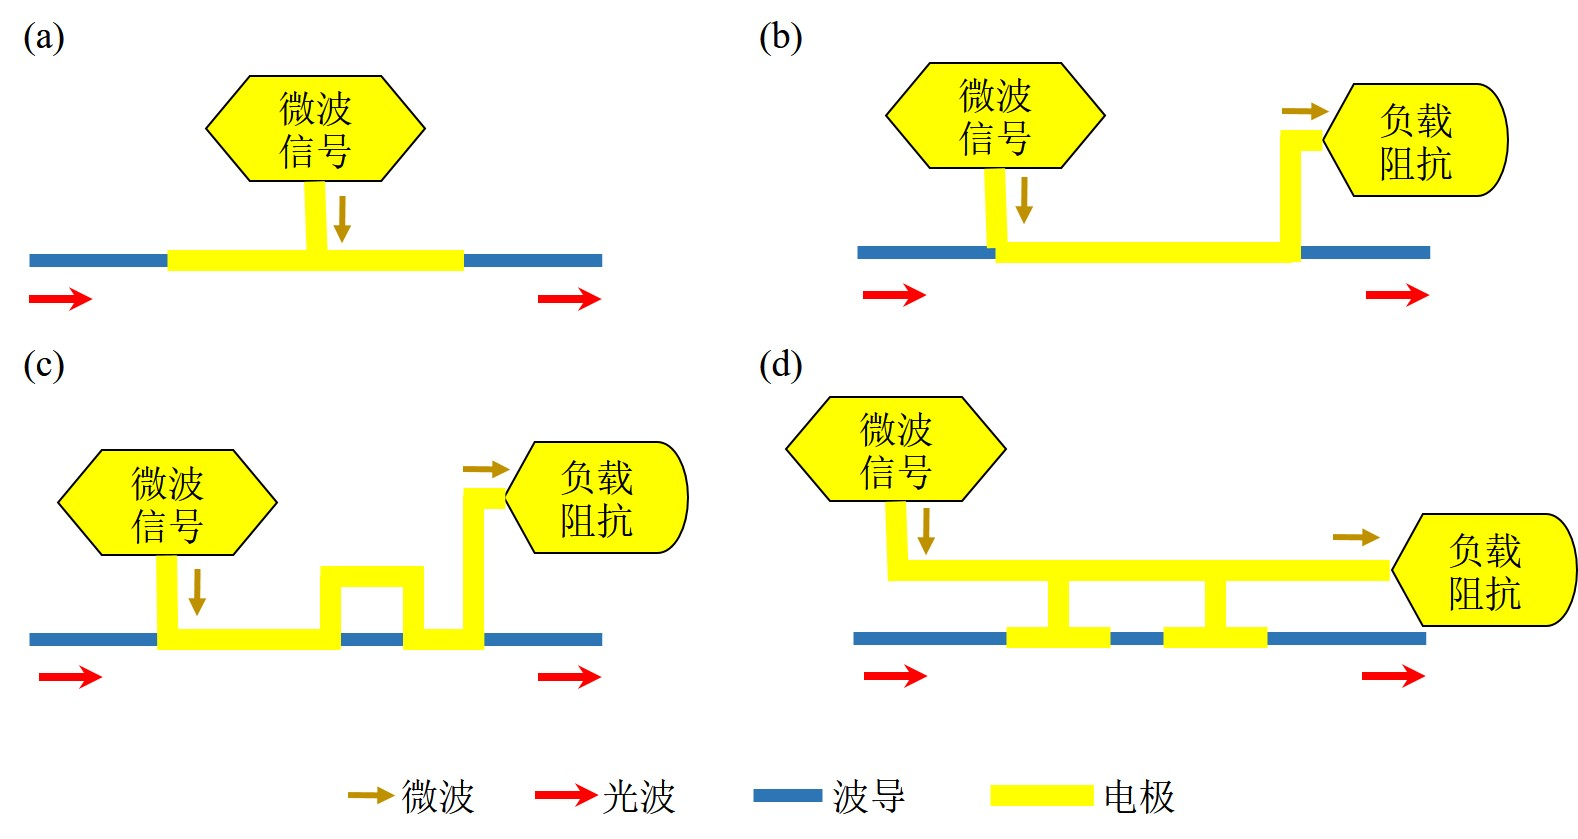
\includegraphics[width=12cm]{./Pictures/fig_mod_ele_type.jpg}
	\caption{ (a) 集总电极;(b)行波电极;(c)分段传输线电极;(d)电容负载行波电极}
	\label{fig_mod_ele_type}
\end{figure}

第一种电极称为集总电极(lumped electrode)如图\ref{fig_mod_ele_type} (a)所示, 这种电极在调制区域的长度小于100 $\mu m$的硅基光调制器中被广泛使用,尤其是小型的谐振型硅基光调制器。由于这类电极末端没有负载是开路,导致微波信号末端反射,集总电极上成为驻波,从而降低所需外界的调制电压,同时也避免了偏置电压在负载上损失的能耗。因此,集总电极在小尺寸,低驱动电压,低能耗的电极上有广泛的应用。图\ref{fig_mod_ele_type_real} (a)展示了集总电极用于InP混合集成到硅波导上的调制器\cite{tang2012energy},实现了低能耗,低驱动电压,小尺寸的调制器。

第二中电极称为行波电极如图\ref{fig_mod_ele_type} (b)所示,这种电极在调制区域大于100 $\mu m$的硅基调制器中被广泛使用,尤其是马赫曾德的硅基光调制器。由于这行波电极调制器需要将电极考虑成为传输线,因此需要设计电极本征阻抗与标准的微波器件的本征阻抗50 $\Omega$相匹配,并且使传输线的传播常数和波导中光的传播常数相匹配,从而尽可能提高调制器的调制带宽。因此,使用行波电极的调制器,在尺寸,驱动电压,能耗上多要高于集总电极的调制器,但是调制速率会有所提高。图\ref{fig_mod_ele_type_real} (b)展示了行波电极用于InP混合集成到硅波导上的调制器\cite{tang2012energy},实现了高速的硅基光调制器。

第三种电极称为分段传输线电极(Segmented Transmission Line Electrode)如图\ref{fig_mod_ele_type} (c)所示, 这种电极也是主要用于调制长度大于100 $\mu m$以上,并且电极的本征电阻和50 $\Omega$相差大,或者微波和光波的传播常数相差较大的硅基光调制器。分段传输线电极是行波电极的一个更为普遍的形式,相比行波电极,其调制带宽可以进一步提高,但是能耗不会有所减少,而尺寸将更进一步增大,。图\ref{fig_mod_ele_type_real} (c)展示了分段传输线电极用于InP混合集成到硅波导上的调制器\cite{tang2012energy},实现了目前调制速度最快的硅基光调制器。

第四种电极称为电容负载行波电极(Capacitively-Loaded Traveling-Wave Electrode)如图\ref{fig_mod_ele_type} (d)所示, 这种电极在硅基光调制器中的应用比较少,主要用于调制长度大于500 $\mu m$以上,并且电极的本征电阻和50 $\Omega$相差大,或者微波和光波的传播常数相差较大的硅基光调制器。由于电容负载行波电极整体和如同行波电极一样,但在单个周期内,调制器区域是集总电极,因此这类电极用于兼顾传输速度和低驱动电压。不过,由于在单个调制器区域还有没参与调制的电极,因此电容负载行波电极的尺寸比较大。图\ref{fig_mod_ele_type_real} (d)展示了电容负载行波电极用于InP混合集成到硅波导上的调制器\cite{tang2012energy},实现了马赫曾德的光调制器。

这四种电极各有优缺点,如果需要尺寸小,能耗低的调制器,可以采用集总电极。如果需要尽可能高的调制速度,或者调制器区域长度比较长时则可以采用行波电极或分段传输线电极结构。而电容负载行波电极是集总电极和分段传输线折中的形式,可以在这两种电极无法满足要求的情况下使用。
\begin{figure}[htb]
	\centering
	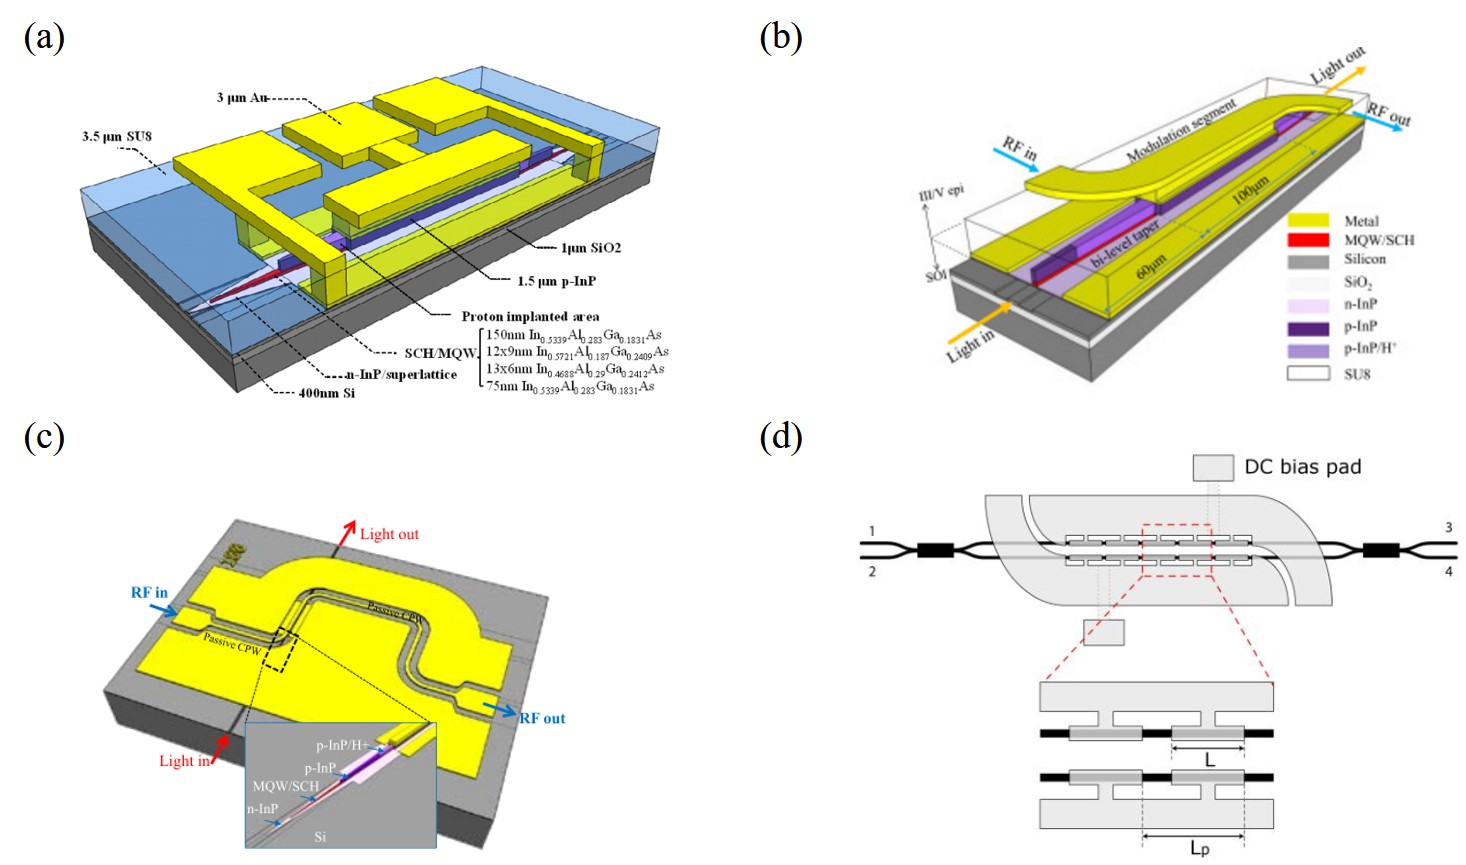
\includegraphics[width=12cm]{./Pictures/fig_mod_ele_type_real.jpg}
	\caption{ (a) 集总电极的实例\cite{tang2012energy};(b)行波电极实例\cite{tang201150};(c)分段传输线电极实例\cite{tang2012over};(d)电容负载行波电极实例\cite{chen2011forty}}
	\label{fig_mod_ele_type_real}
\end{figure}


\subsection{纯硅基光调制器}
\subsection{硅基混合集成III-V光调制器}
\subsection{硅基聚合物光调制器}
\subsection{硅基外延锗硅光调制器}
\subsection{硅基石墨烯光调制器}
\subsection{硅基铌酸锂光调制器}
\subsection{硅基钛酸钡光调制器}
\subsection{硅基压电陶瓷光调制器}
\subsection{硅基基于表面等离子体波导的光调制器}
\subsection{硅基单光子调制器}
\subsection{国内硅基光调制器的进展}
\section{论文的内容和创新点}

\subsection{论文内容}
\subsection{论文创新点}


